
\documentclass[conference]{IEEEtran}
\ifCLASSINFOpdf
  \usepackage[pdftex]{graphicx}
\hyphenation{op-tical net-works semi-conduc-tor}


\begin{document}
\title{Decision Tree based Classifiers with GA based feature selectors}


% author names and affiliations
% use a multiple column layout for up to three different
% affiliations
\author{
\IEEEauthorblockN{Samir Sheriff}
\IEEEauthorblockA{BE 7 semester\\ Department of Computer Science\\RV College of Engineering\\
Email:samiriff@gmail.com}
\and
\IEEEauthorblockN{Satvik N}
\IEEEauthorblockA{BE 7 semester\\ Department of Computer Science\\RV College of Engineering\\
Email:nsatvik@gmail.com}
\and
\IEEEauthorblockN{Mrs. Shanta Rangaswamy }
\IEEEauthorblockA{Assistant Professor\\ Department of Computer Science\\RV College of Engineering\\
Email:shantharangaswamy@rvce.edu.in}
}




% make the title area
\maketitle


\begin{abstract}
%\boldmath
Virtualization is the buzz word in today\'s IT. Virtualization provides high availability for critical applications, and streamlines application deployment and migrations.

 
Virtualization has become an essential technology in the data center. Virtualization improves resource utilization through server consolidation, but it also makes resource management more complex. 


Virtualization can simplify IT operations and allow IT organizations to respond faster to changing business demands. This paper discusses the different resource management  techniques recently developed and researched by researchers that are applied on Virtual machines to achieve maximium throughput, minimize response time, and avoid overload.
\end{abstract}
\begin{keywords}
decision tree, machine learning, genetic algorithms, decision problems.
\end{keywords}

\IEEEpeerreviewmaketitle



\section{Introduction}


\textbf{Virtualization} is the abstraction of IT resources that masks the physical nature and boundaries of those resources from resource users. An IT resource can be a server, a client, storage, networks, applications or OSs. Essentially, any IT building block can potentially be abstracted from resource users. At one time, virtualization was considered just an academic interest. But now, it is used widely in the industry to provide cost effective and flexible applications. 


Allocation of resources in a virtual environment holds the key in the performance of virtual machines. The main  resources of a virtual machine include CPU, memory, disk, and network resources. Each virtual machine consumes a portion of the CPU, memory, network bandwidth, and storage resources of the physical machine it belongs to.\\
The host guarantees each virtual machine, its share of the underlying hardware resources based on a number of factors.
\begin{enumerate}
\item{Available resources for the physical machine}
\item{Reservation, limit, or shares of the virtual machine.}
\item{Number of virtual machines powered on, and resource utilization by those virtual
machines.}
\item{Overhead required to manage the virtualization.}
\end{enumerate}
Effective management of virtualized resources is a challenging task for providers, as it often involves selecting the best resource allocation out of a large number of alternatives. In the following sections we discuss various resource management techniques in virtual environment.



\section{Resoure Management Techniques}
In this section, we talk about three important resource management techniques employed in virtual environment.
\subsection{Replication and Migration as Resource Management Mechanisms}
Virtualization refers to an abstract layer between the operating system and the hardware. The layer provides an interface to the actual hardware that allows for the support of a number of virtual machines. A Virtual machine running a server program is called an virtual server.\\



Due to virtualization, the applications get smaller portion of the physical hardware. Thus virtualization benefits the data centers by allowing several applications to make use of a physical machine. This suggests that resource allocation should be dynamic to
support the allocation of resources on-demand.


Dynamic resource management requires \textbf{monitoring mechanisms} and \textbf{dynamic resource reallocation mechanisms}. Examples of this mechanisms are migration and replication which are included under virtual server relocation. \textbf{Migration} consists of transferring a running virtual machine from one physical machine to another. \textbf{Replication} entails the creation of a replica of a virtual machine on another physical machine. Requests for the virtual server are balanced between the two instances. This should reduce the computing resources needed by a single physical machine by distributing requests to two different virtual machines on two different physical machines.\\
This technique is useful when the the combined resource needs of the virtual machines hosted in a physical machine exceed the resource availability.



In this paper the authors use OpenVZ which provides operating
system-level virtualization. OpenVZ is a Linux kernel modified to run multiple, isolated containers (i.e., virtual user-space environments) on a single physical  machine or hardware node. OpenVZ supports the execution of multiple containers. The containers are isolated program execution environments, which appear as stand-alone servers to users. The host system runs inside a privileged container.


\textbf{System Design} 


Golondrina was conceived as a multi-resource management system for data centers. Golondrina consists of three primary management entities: \textbf{Client, Server, Gate}.

\begin{figure}[h!]
  \centering
   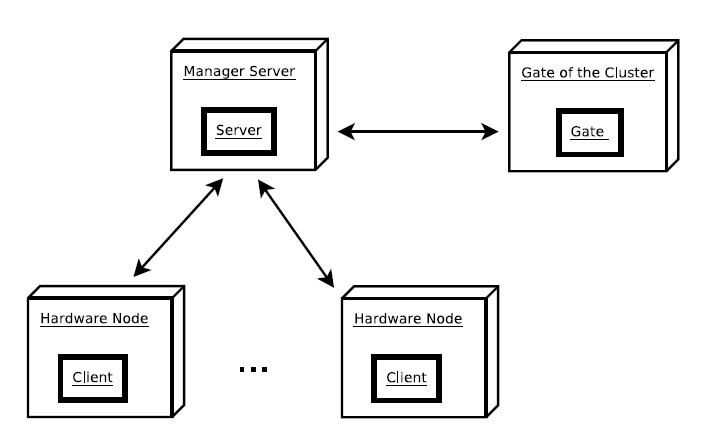
\includegraphics[scale=0.50]{Golondrina.png}
  \caption{Golondrina's system architecture.}
\end{figure}

\begin{enumerate}
\item{\textbf{Client}} - Each hardware node has a Client instance that runs in the privileged container. The Client requires access to the operating system’s configuration and accounting files, and the OpenVZ management tools. The Client instance provides
the following functionality:
\begin{enumerate}
\item{The periodic collection of CPU utilization statistics from the containers and the hardware node. This is done by reading the hardware node’s
operating system’s accounting files through the proc file system. These statistics are sent to the Server.}
\item{Support for migration and replication of the containers. This is done upon a request from the Server.}
\end{enumerate}
\item{\textbf{Server}} Upon receiving the CPU utilization statistics sent by the Client, the Server stores the statistics. The data model used assumes that the hardware node is an aggregation of containers. The attributes of the hardware node and containers represent CPU utilization metrics. 
\begin{enumerate}
\item{\textbf{Analyzing CPU Utilization Statistics}} The CPU utilization statistics sent by the client are used to create a CPU utilization profile of resource usage over time. A mathematical
model uses the CPU utilization statistics collected at time $t_i$ for predicting the CPU utilization of a container or hardware node at time $t_{i+1}$.
This mathematical model relies on the last observation in the sequence of observations and two parameters: $\mu$, the mean of the values in the sequence, and $\theta$, which accounts for the variations of the values in the sequence. 

Given a sliding window of CPU utilization statistics W = [$u_x, ..., u_t$] with maximum size w and where x = max(0, t-w + 1). The parameters $\mu$ and $\theta$ at time t are calculated as
follows:
$$\mu_t = \frac{\sum_{i=x}^{t}u_i}{t-x+1}$$
$$\theta_t = \frac{\sum_{i=x}^{t-1}(u_i -\mu_t)\ast(u_{i+1}-\mu_t)}{max(1,\sum_{i=x}^{t-1}(u_i-\mu_t)^{2})}$$

Having the values $u_t, \mu_t and \theta_t$, it is possible to predict
the CPU utilization at time t + 1:
$$u_{t+1} = \mu_t + \theta_t * (u_t - \mu_t)$$
The profiling process uses a historical policy to calculate the container’s profiled CPU utilization. 

\item{\textbf{Resource Stress Check}} The Server executes a resource stress check on every hardware node that is not currently involved in a relocation. 
The resource stress check consists of two steps. First, it verifies whether the predicted CPU utilization of the hardware node exceeds the CPU utilization threshold. Then, if the latter is true, it checks whether k out of the previous n resource stress checks also exceeded the threshold, in which case the hardware node is considered to be under a resource stress situation.

$$(u_{t+1} > threshold) \land (\sum_{i=1}^{n}(u_i > threshold)\geq k)$$
\item{\textbf{Reloation Search}} 


 After the resource stress check round is completed the hardware nodes are classified as stressed or non-stressed hardware nodes. If both sets are non-empty, then the Server searches for a sequence of relocations to solve the resource stress situations. This decision making process consists of determining which containers hosted in stressed hardware nodes will be relocated and which non-stressed hardware nodes will serve as a target for those relocations.

\end{enumerate}


\item{\textbf{Gate}} The Gate component runs in a non-virtualized physical server, which is used as the gate of the cluster (i.e., all service requests come through this physical server). Its responsibility is to update the load balancer’s configuration after a replication occurs.
\end{enumerate}


\subsection{Autonomic resource management using
fuzzy logic-based approaches}

In this paper the author proposes a two-level resource management
system to dynamically allocate resources to individual
virtual containers. It uses local controllers at the virtual container
level and a global controller at the resource-pool
level. An important advantage of this two-level control architecture
is that it allows independent controller designs for
separately optimizing the performance of applications and
the use of resources. Autonomic resource allocation is realized
through the interaction of the local and global controllers.

\begin{figure}[h!]
  \centering
   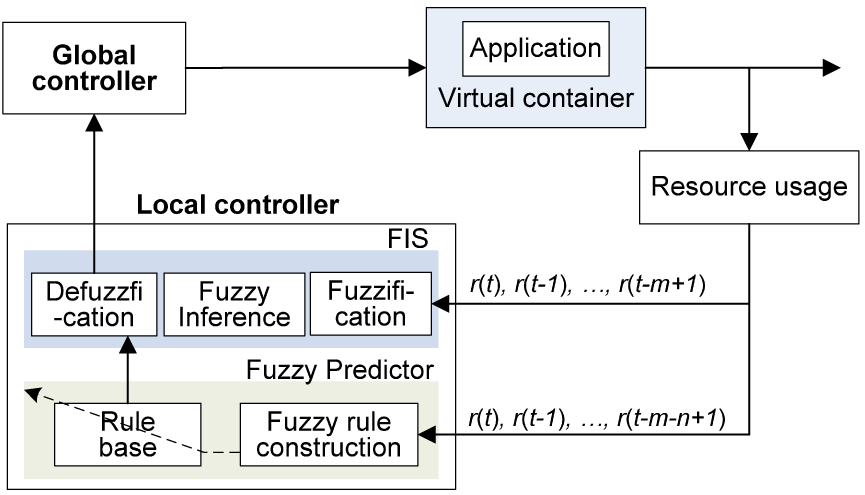
\includegraphics[scale=0.30]{fuzzy_block_dia.png}
  \caption{Resource management based on fuzzy logic systems.}
\end{figure}

Local controller uses fuzzy logic-based approaches to efficiently and robustly deal with the complexity and uncertainties of dynamically
changing workloads and resource usage. The global controller
determines the resource allocation based on a proposed
profit model, with the goal of maximizing the total
profit of the data center. This resource
management system can significantly reduce resource consumption
while still achieving application performance targets. Resource
management in a data center is decoupled at two levels:
virtual containers and resource pools. The key to cost effective
resource allocation is the ability to efficiently find
the minimum amount of resources that an application needs
to meet the desired QoS.





In each virtual container hosting an
application, a local controller is responsible for determining
the amount of resources needed by the application and making
resource requests accordingly. A global controller responds
to the local controllers’ requests by dynamically allocating
resources across multiple virtual containers hosted
on the same physical resources. It controls the resource allocations
in a way that maximizes the data center’s profit.




Two fuzzy-logic-based approaches - fuzzy modeling and
fuzzy prediction are proposed for use by local controllers
in automatically learning of runtime behavior of virtual containers
under dynamically changing workloads. Two-level resource control system is preferred over
the more obvious centralized approach in which all the control
functions are implemented at one centralized location.
Since local containers are independent of each other, heterogeneous
local controllers’ implementations are possible
The system handles two different types of
optimizations independently. 




Interaction between the local and global controllers enables
a virtual container to augment its resources in response to
increased workload, and to reduce its resources when they
are no longer needed. The main task of the local controller
is to estimate the set of resources needed by an application
running in the container. Each individual local controller tries to minimize the resource
cost by only requesting the resources necessary for meeting the application SLA. 



The global controller receives requests for physical resources from the local controllers and allocates the resources among them as required. It seeks to make allocations that maximize the data center’s profit, which is the revenue received by allocating the physical resources
among virtual containers minus the penalties due to violations of resource SLA.

\begin{figure}[h!]
  \centering
   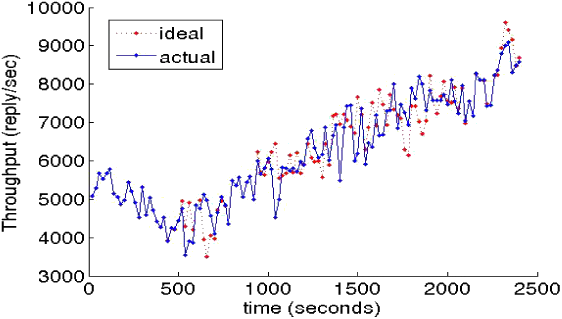
\includegraphics[scale=0.50]{fuzzy_experiment.png}
  \caption{Experimental Results}
\end{figure}
A real world experiment was conducted using the Fuzzy Approach. The results were promising. Figure 3 shows that the application’s throughput achieved by using the local controller is close to the ideal throughput obtainable for the
workload (the difference is within 5\%), indicating the effectiveness of the fuzzy-modeling approach under real-world
workloads\\
\textbf{\emph{Advantages Of Fuzzy Based Method}}:
One of the advantages of fuzzy approaches is that they do not require prior knowledge or a mathematical model of the system being managed. They typically do not need time-consuming training, which makes them suitable for real-time control. Moreover, the approaches are robust with respect to noisy data and have the ability to adapt to changes very quickly


\subsection{Sandpiper-Black Box and Gray box resource management technique}
This paper studies automated black-box and gray-box strategies for virtual machine provisioning in large data centers. These techniques automate the tasks of monitoring system resource usage, hotspot detection, allocating resources and initiating any necessary migrations. More importantly, the black-box techniques can make decisions by simply observing each virtual
machine from the outside and without any knowledge of the application resident within each VM. The authors also present a gray-box approach that assumes access to a small
amount of OS-level statistics in addition to external observations
to better inform the provisioning algorithm. The authors have designed and implemented the Sandpiper system to support either black-box, gray-box, or combined
techniques. They have identified specific limitations of the
black-box approach and understood how a gray-box approach
can address them.


Sandpiper implements a hotspot detection algorithm
that determines when to resize or migrate virtual machines,
and a hotspot mitigation algorithm that determines what
and where to migrate and how many resources to allocate.
The hotspot detection component employs a monitoring
and profiling engine that gathers usage statistics on various
virtual and physical servers and constructs profiles of
resource usage. These profiles are used in conjunction with
prediction techniques to detect hotspots in the system.
Upon detection, Sandpiper grants additional resources to
the overloaded servers if available. If necessary, Sandpiper’s migration manager is invoked for further hotspot
mitigation. The migration manager employs provisioning
techniques to determine the resource needs of overloaded
VMs and uses a greedy algorithm to determine a sequence
of moves or swaps to migrate overloaded VMs to underloaded
servers.



Sandpiper supports both black- and gray-box monitoring
techniques that are combined with profile generation
tools to detect hotspots and predict VM resource
requirements.

\begin{figure}[h!]
  \centering
   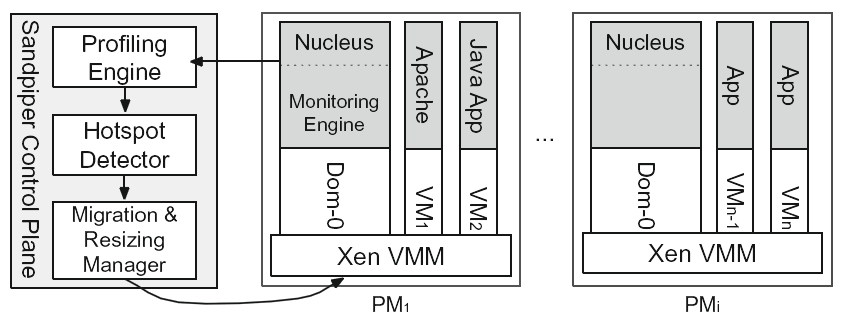
\includegraphics[scale=0.30]{sandpiper_arch.png}
  \caption{The Sandpiper architecture.}
\end{figure}

\begin{enumerate}
\item{\textbf{Unobtrusive black-box monitoring}} The monitoring engine is responsible for tracking the processor, network and memory usage of each virtual server.
It also tracks the total resource usage on each physical
server by aggregating the usages of resident VMs.
In a pure black-box approach, all usages must be inferred
solely from external observations and without relying
on OS-level support inside the VM

\item{\textbf{CPU Monitoring}} By instrumenting a hypervisor,
it is possible to gain access to CPU
scheduling events which indicate when a VM is scheduled
and when it relinquishes the CPU. These events are tracked
to determine the duration for which each virtual machine
is scheduled within each measurement interval.

\item{\textbf{Network Monitoring}} The monitoring engine can conveniently
monitor each VM’s network usage. The monitoring engines can use the Linux /
proc interface to monitor the number of bytes sent and received on each interface.
These statistics are gathered over interval I and returned
to the control plane.

\item{\textbf{Memory Monitoring}} Black-box monitoring of memory
is challenging since Xen allocates a user-specified amount
of memory to each VM and requires the OS within the VM
to manage that memory; as a result, the memory utilization
is only known to the OS within each VM. It is possible
to instrument Xen to observe memory accesses within
each VM through the use of shadow page tables, which is
used by Xen’s migration mechanism to determine which
pages are dirtied during migration. However, trapping each
memory access results in a significant application slowdown
and is only enabled during migrations[6]. Thus,
memory usage statistics are not directly available and
must be inferred.


\end{enumerate}


\textbf{Gray-box monitoring}




Sandpiper supports gray-box monitoring, when feasible,
using a light-weight monitoring daemon that is installed
inside each virtual server. In Linux, the monitoring daemon uses the /proc interface to gather OS-level statistics of CPU, network, and memory usage.
The memory usage monitoring, in particular, enables proactive
detection and mitigation of memory hotspots. The
monitoring daemon also can process logs of applications
such as web and database servers to derive statistics such
as request rate, request drops and service times. Direct
monitoring of such application-level statistics enables explicit
detection of SLA violations, in contrast to the blackbox
approach that uses resource utilizations as a proxy
metric for SLA monitoring.


\textbf{Profile generation} 



The profiling engine receives periodic reports of resource
usage from each nucleus. It maintains a usage history
for each server, which is then used to compute a
profile for each virtual and physical server. A profile is a
compact description of that server’s resource usage over
a sliding time window W. Three black-box profiles are
maintained per virtual server: CPU utilization, network
bandwidth utilization, and swap rate (i.e., page fault rate).
If gray-box monitoring is permitted, four additional profiles
are maintained: memory utilization, service time, request
drop rate and incoming request rate. Similar
profiles are also maintained for each physical server, which
indicate the aggregate usage of resident VMs.


\textbf{Hotspot detection}




The hotspot detection algorithm is responsible for signaling
a need for VM resizing whenever SLA violations
are detected implicitly by the black-box approach or
explicitly by the gray-box approach. Hotspot detection is
performed on a per-physical server basis in the black-box
approach.



\textbf{Resource provisioning}



A hotspot indicates a resource deficit on the underlying
physical server to service the collective workloads of resident
VMs. Before the hotspot can be resolved, Sandpiper must first estimate how much additional resources are
needed by the overloaded VMs to fulfill their SLAs.




\textbf{Hotspot mitigation}



Once a hotspot has been detected, Sandpiper must
determine if the hotspots can be resolved with local resource
adjustments, or if migrations are required to balance
load between hosts 



% An example of a floating figure using the graphicx package.
% Note that \label must occur AFTER (or within) \caption.
% For figures, \caption should occur after the \includegraphics.
% Note that IEEEtran v1.7 and later has special internal code that
% is designed to preserve the operation of \label within \caption
% even when the captionsoff option is in effect. However, because
% of issues like this, it may be the safest practice to put all your
% \label just after \caption rather than within \caption{}.
%
% Reminder: the "draftcls" or "draftclsnofoot", not "draft", class
% option should be used if it is desired that the figures are to be
% displayed while in draft mode.
%
%\begin{figure}[!t]
%\centering
%\includegraphics[width=2.5in]{myfigure}
% where an .eps filename suffix will be assumed under latex, 
% and a .pdf suffix will be assumed for pdflatex; or what has been declared
% via \DeclareGraphicsExtensions.
%\caption{Simulation Results}
%\label{fig_sim}
%\end{figure}

% Note that IEEE typically puts floats only at the top, even when this
% results in a large percentage of a column being occupied by floats.


% An example of a double column floating figure using two subfigures.
% (The subfig.sty package must be loaded for this to work.)
% The subfigure \label commands are set within each subfloat command, the
% \label for the overall figure must come after \caption.
% \hfil must be used as a separator to get equal spacing.
% The subfigure.sty package works much the same way, except \subfigure is
% used instead of \subfloat.
%
%\begin{figure*}[!t]
%\centerline{\subfloat[Case I]\includegraphics[width=2.5in]{subfigcase1}%
%\label{fig_first_case}}
%\hfil
%\subfloat[Case II]{\includegraphics[width=2.5in]{subfigcase2}%
%\label{fig_second_case}}}
%\caption{Simulation results}
%\label{fig_sim}
%\end{figure*}
%
% Note that often IEEE papers with subfigures do not employ subfigure
% captions (using the optional argument to \subfloat), but instead will
% reference/describe all of them (a), (b), etc., within the main caption.


% An example of a floating table. Note that, for IEEE style tables, the 
% \caption command should come BEFORE the table. Table text will default to
% \footnotesize as IEEE normally uses this smaller font for tables.
% The \label must come after \caption as always.
%
%\begin{table}[!t]
%% increase table row spacing, adjust to taste
%\renewcommand{\arraystretch}{1.3}
% if using array.sty, it might be a good idea to tweak the value of
% \extrarowheight as needed to properly center the text within the cells
%\caption{An Example of a Table}
%\label{table_example}
%\centering
%% Some packages, such as MDW tools, offer better commands for making tables
%% than the plain LaTeX2e tabular which is used here.
%\begin{tabular}{|c||c|}
%\hline
%One & Two\\
%\hline
%Three & Four\\
%\hline
%\end{tabular}
%\end{table}


% Note that IEEE does not put floats in the very first column - or typically
% anywhere on the first page for that matter. Also, in-text middle ("here")
% positioning is not used. Most IEEE journals/conferences use top floats
% exclusively. Note that, LaTeX2e, unlike IEEE journals/conferences, places
% footnotes above bottom floats. This can be corrected via the \fnbelowfloat
% command of the stfloats package.



\section{Conclusion}
The study in [2] proposes a resource management system for operating system level virtualized environments. In addition, this is the first c study that uses replication as an alternative to migration
and compares both mechanisms.
There are many ways in which the Golondrina could be extended. One of them is adding memory and network as managed resources. 





The paper [4] argued that virtualization provides significant
benefits in data centers by enabling virtual machine
migration to eliminate hot spots.The authors introduced Sandpiper,  system that automates the task of monitoring and detecting
hotspots, determining a new mapping of physical to
virtual resources, and resizing or migrating VM’s to eliminate
the hotspots. They discussed a black-box strategy that
is fully OS- and application-agnostic as well as a graybox
approach that can exploit OS- and application-level
statistics. An evaluation of their Xen-based prototype
showed that VM migration is a viable technique for rapid
hotspot elimination in data center environments. Using solely
black-box methods, Sandpiper was capable of eliminating
simultaneous hotspots involving multiple resources.
They found that utilizing gray-box information can improve
the responsiveness of our system, particularly by allowing
for proactive memory allocations and better inferences
about resource requirements.




% conference papers do not normally have an appendix


% use section* for acknowledgement
%\section*{Acknowledgment}


%The authors would like to thank...





% trigger a \newpage just before the given reference
% number - used to balance the columns on the last page
% adjust value as needed - may need to be readjusted if
% the document is modified later
%\IEEEtriggeratref{8}
% The "triggered" command can be changed if desired:
%\IEEEtriggercmd{\enlargethispage{-5in}}

% references section

% can use a bibliography generated by BibTeX as a .bbl file
% BibTeX documentation can be easily obtained at:
% http://www.ctan.org/tex-archive/biblio/bibtex/contrib/doc/
% The IEEEtran BibTeX style support page is at:
% http://www.michaelshell.org/tex/ieeetran/bibtex/
%\bibliographystyle{IEEEtran}
% argument is your BibTeX string definitions and bibliography database(s)
%\bibliography{IEEEabrv,../bib/paper}
%
% <OR> manually copy in the resultant .bbl file
% set second argument of \begin to the number of references
% (used to reserve space for the reference number labels box)
\begin{thebibliography}{1}

\bibitem{textbook}
Lutfiyya; Hanan, Keller; Gaston.
\emph{Replication and Migration as Resource Management Mechanisms for Virtualized Environments.}
2010, Sixth Internation Conference on Autonomic and Autonomous Systems.
\bibitem{paper}
Jing Xu, Ming Zhao,José Fortes, Robert Carpenter,
Mazin Yousif. \emph{Autonomic resource management in virtualized data centers using
fuzzy logic-based approaches} Cluster Comput (2008) 11: 213–227
DOI 10.1007/s10586-008-0060-0
\bibitem{paper}
T. Wood et al., \emph{Sandpiper.Black-box and gray-box resource management for virtual machines}, Computer Network (2009), doi:10.1016/j.comnet.2009.04.014


\end{thebibliography}




% that's all folks
\end{document}


